\chapter{Analyse}
In diesem Kapitel wird die Problemlage im Bezug zum derzeitigen Stand der Technik analysiert.
Etablierte Verfahren werden mithilfe eines geeigneten Testdatensatzes anschließend evaluiert.
Das geeignetste Verfahren wird für den weiteren Verlauf der Arbeit bestimmt.
* Vorarbeit -> Ausarbeiten des bestmöglichen Algorithmus\newline

* Verkehrskameras laden\newline
* Verkehrsbilder laden über Verkehrskameras\newline
* Auswahl verschiedener Ansätze\newline
* Vergleich der Ansätze in Bezug auf Ressourcenlast und Effizienz bzw. Effektivität\newline
* Datensätze generieren, um Vergleichskriterien zu erstellen\newline

\section{Stand der Technik}
Bildverarbeitung ist ein Thema, dass schon sehr lange im Bereich der Informationstechnik und Informatik erforscht wird.
Besonders durch derzeitige Entwicklungen in der künstlichen Intelligenz und der Objekterkennung bekommt das Thema in der heutigen Zeit eine hohe Bedeutung für die technische Entwicklung. Im folgenden Kapitel werden einige der zum derzeitigen Zeitpunkt etablierten Verfahren der Bildverarbeitung im Kontext der Aufgabenstellung evaluiert und bewertet.

\subsection{Statische Verfahren}
Verfahren, welche ohne einen speziellen Kontext direkt auf die Pixelwerte eines Bildes angewendet werden können, werden im folgenden als "`statische Verfahren"' beschrieben. In den meisten Fällen sind diese Verfahren besonders ressourceneffizient, da sie mit weniger Speicher- und Zeitkomplexität auskommen.
\subsubsection{Statische Pixel Analyse}
Ein trivialer Ansatz um Veränderungen zwischen zwei oder mehreren Bildern zu erkennen kann durch einen Vergleich der Pixelwerte ermöglicht werden.
So ist es auch möglich Pixelwerte eines einzigen Bildes zu analysieren und somit beispielsweise bestimmte Helligkeits- oder Farbveränderungen  im Bild festzustellen.
Die beschriebenen Helligkeits- oder Farbwechsel können im Bezug zur Objekterkennung auf einem Bild verwendet werden, indem man die jeweiligen Pixelwerte mit denen des Hintergrundes im Bild vergleicht.
Für den Fall der Verkehrskameras würde der besagte Hintergrund die Pixelwerte der Straße in dem gewählten Bereich beschreiben.
Sobald eine Reihe von Pixeln durch einen starken Farb- oder Intensitätswertwechsel unterbrochen wird, kann man in diesem Fall von einem beweglichen Objekt auf der Straße ausgehen.
Bin O.K. Rahmat und bin Jumari beschreiben in ihrer Arbeit \cite{bin2001vehicle} ein solches Verfahren und wenden dies auf Bilder von Verkehrskameras an. 
Die Besonderheit ist hierbei, dass nicht alle Pixelwerte des Bildes verglichen werden, sondern nur ein relevanter Teilabschnitt zu Vergleichszwecken ausgesucht wird. 
Dieser Teilbereich wird von den Autoren auch als "`Detektor"' beschrieben und befindet sich komplett auf der ausgewählten Fahrbahn.
Die Länge eines stockenden Verkehrsflusses kann ebenfalls über diese Methode ermittelt werden. 
Hierfür wird in der Arbeit der beiden Autoren ein länglicher Detektor verwendet der sich über den kompletten im Bild ersichtlichen Streckenabschnitt zieht.
Weiterhin werden die Farbwechsel innerhalb der Detektoren ausgewertet, um die einzelnen Objekte voneinander zu trennen.
Das Verfahren hat eine sehr geringe Komplexität und ist daher einfach zu implementieren, jedoch werden auch schon in der Arbeit Situationen beschrieben in denen das Verfahren keine zuverlässigen Ergebnisse liefert. 
So kann zum Beispiel der Lichtkegel eines Scheinwerfers bei Nacht das Ergebnis verfälschen.
\subsubsection{Kantenerkennung}
Kantenerkennung bezeichnet eine Klasse von Verfahren, bei welchen Kanten im Bild über abrupte Intensitätswert-Übergänge gefunden werden. 
Dabei werden in der Regel Faltungskerne (siehe \ref{sec:Faltungskerne}) verwendet, um die Ableitung der Intensitätswert-Funktion in einem Grauwert-Bild zu ermitteln (Abbildung~\ref{fig:gupte1}).
Das bedeutet man muss für die Anwendung des Verfahrens das Bild in den Grauwert-Bereich übertragen.
Die Kanten können dann anschließend für die Objekterkennung verwendet werden. Um leicht überlagernde Objektkanten voneinander zu trennen können morphologische Operatoren verwendet werden (siehe \ref{sec:MorphologischeOperatoren}).
Gupte und Papanikolopoulos stellen ein solches Verfahren in \cite{gupte2000algorithms} vor. Dabei werden Kanten auf zwei Bildern einer Verkehrskamera erkannt und dann beide Kantenbilder per XOR vereinigt. Das Ergebnis wird anschließend mithilfe von der Anwendung von mehreren Dilatation-Operationen verbessert, da nicht geschlossene und im Objekt liegende Kanten zur einer großen Kante verbunden werden (Abbildung~\ref{fig:gupte2}).
Dieses Verfahren ist ebenfalls wenig komplex und lässt sich einfach implementieren. 
Jedoch besitzt es auch einige Nachteile, wie zum Beispiel, dass sich Schattenwurf negativ auf das Ergebnis auswirkt und eine Perspektive im Bild vorausgesetzt wird.

\begin{figure}[ht]
  \centering
	\begin{minipage}[b]{0.4\textwidth}
     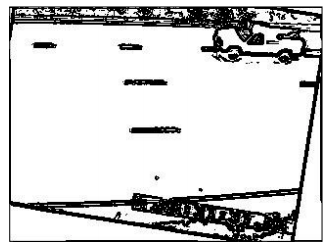
\includegraphics[width=\textwidth]{Bilder/gupte1} \\
   \caption{Kantenerkennung}
   \label{fig:gupte1}
  \end{minipage}
	\hfill
	\begin{minipage}[b]{0.4\textwidth}
     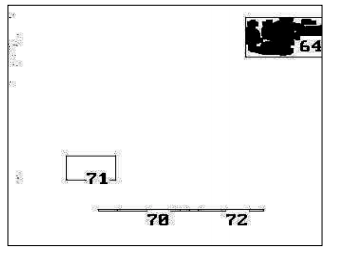
\includegraphics[width=\textwidth]{Bilder/gupte2} \\
		\caption{Ergebnis des Verfahrens}
		\label{fig:gupte2}
	\end{minipage}
\end{figure}
\newpage

\subsection{Dynamische Verfahren}
Als "`dynamische Verfahren"' werden im folgenden Verfahren beschrieben, die nur innerhalb eines bestimmten Kontextes auf ein Bild angewendet werden sein. So kann es sein, dass das Verfahren bestimmte Trainingsdaten oder Vergleichswerte von anderen Bildern benötigt. Dies erhöht in den meisten Fällen die Genauigkeit des Verfahrens, aber die Ressourceneffizienz wird drastisch verringert.
\subsubsection{Neuronale Netze}
Neuronale Netze sind ein Beispiel für Verfahren aus dem maschinellen Lernen. 
Die Arbeit \cite{hkkDhbw} geht im Detail darauf ein wie das Problem der Stauerkennung auf Bildern mithilfe eines konvolutionalen neuronalen Netzwerks gelöst werden kann. 
Jedoch fällt bei Laufzeit eines komplexen neuronalen Netzes auf, dass das Laden und Benutzen der interne Zustandsmaschine einen relativ hohen Hauptspeicher-Bedarf mit sich bringt.
Der Vorteil der sich jedoch hierdurch bietet ist, dass Bilder nicht statisch analysiert werden, sondern das Netz dynamisch auf Bilder und Verhältnisse, wie zum Beispiel Perspektive und Wetter, trainiert wird.
Dieses Verfahren wurde für die folgende Implementierung nicht gewählt, da diese Arbeit einen besonderen Fokus auf die Ressourcensparsamkeit des Verfahrens setzt.
* Gewählter Ansatz des letzten Jahrgangs\newline
* Vermutlich bester Ansatz, da keine statische Analyse der Bilder durchgeführt wird\newline
	sondern dynamisch auf konkrete Bilder und Verhältnisse (Perspektive und Situation) trainiert wird
* Nicht durchgeführt, da feststand, dass der Ansatz zu Ressourcenintensiv ist und Ziel der Arbeit war Ressourcen zu sparen\newline

\subsubsection{Background Subtraction}
Background Subtraction, auch als Foreground Detection bekannt, ist eine Klasse von Verfahren, bei denen einer Serie von Bildern analysiert wird, um Objekte im Vordergrund des Bildes vom Hintergrund zu trennen. 
Hierfür wird ein sogenanntes Hintergrund-Modell aus den ersten Bilder der Serie generiert, welches dann auf das letzte Bild angewandt wird, um ein Objekt im Vordergrund zu erkennen.
In dem Artikel \cite{mcivor2000background} werden mehrere dieser Hintergrund-Modelle im Detail beschrieben.
Bei der Auswahl des geeigneten Hintergrund-Modells sind mehrere Parameter zu berücksichtigen, wie zum Beispiel Perspektive und Farb- und Intensitäts-Spektrum.
Akoum beschreibt im Artikel \cite{akoumBSIP} wie das Hintergrund-Modell "`Gaussian mixture Models"', oft auch als "`Mixtures of Gaussians"' beschrieben, auf ein Video einer Verkehrskamera angewandt werden kann.
Objekte die im Bild durch das Verfahren erkannt wurden sind im Anschluss weiß eingefärbt, während der Hintergrund schwarz eingefärbt wird.
Das Ergebnis des Verfahrens wird mit Dilatations- und Erosions-Filtern im Anschluss verbessert. 
Der Dilatations-Filter sorgt dabei für die Verbindung von nicht geschlossenen Kanten, während der Erosions-Filter kleine unwichtige Kanten aus dem Bild entfernt.
Das Verfahren ist relativ komplex, bietet dafür aber eine sehr gute Genauigkeit. 
Weiterhin gibt es bereits einige Implementierungen diverser Hintergrund-Modelle in der Bibliothek OpenCV (siehe \ref{sec:OpenCV}).

\section{Bestimmung des Testdatensatzes}
\subsection{Verkehrskameras laden}
\label{sec:AnaCam}
Bevor die Kamerabilder geladen werden können, ist es zunächst relevant zu wissen welche Kameras es überhaupt gibt und wo diese liegen.
Hierfür stellt die Verkehrszentrale eine Liste aller Kameras unter dieser Webadresse bereit: \url{http://www.svz-bw.de/kamera/kamera_A.txt} (Stand: 31.3.2019).

Diese liegen in einer durch Leerzeichen separierten Tabellenstruktur vor.

\begin{center}
\scriptsize
    \begin{tabular}{ | l | l | l | l | l | l | l | l |}
    \hline
		lon & lat & title & description & linkextern & icon & iconSize & iconOffset \\ \hline
    572330.13 &
		5361095.33 &
		... &
		/.../kameradetail.php?id=EXT006 &
		... &
		... &
		16,16 &
		-8,-8 \\
    \hline
    \end{tabular}
\end{center}

Die Werte {\em lat} und {\em lon} beschreiben die Position der Kamera durch Längen und Breitengrad.
Der Eintrag {\em title} enthält einen ausfühlicheren Titel der Kamera. Mit {\em description} hat man die Möglichkeit eine detailiertere Beschreibung der Kamera zu erhalten, welche jedoch mit HTML Tags angereichert ist. {\em Linkextern} ist die Webadresse, über welche auf die Kamera zugegriffen werden kann. {\em Icon}, {\em iconSize} und {\em iconOffset} sind Informationen, die das Straßenverkehrszentrum selbst benötigt, um das Kameraicon auf einer Landkarte anzuzeigen.

Relevant sind also zunächst die Koordinaten, der Titel und der Link, da nur über diesen die ID der Kamera aufgelöst werden kann.
Das erste Problem hierbei ist, dass die Koordinaten der Kamera nicht der üblichen Projektion der Weltkugel entsprechen. Gebräuchlich ist die Projektion {\em WGS 84}~\cite{wgs84}, welche auch von Navigationssystemen oder herkömlichen Kartendiensten genutzt wird und den Globus von -180° westlich bis 180° nördlich, bzw. -90° südlich bis 90° nördlich einteilt.

Das Straßenverkehrszentrum nutzt jedoch das Referenzsystem {\em ETRS89 / UTM zone 32N}~\cite{etrs89}, welches für Europa ausgelegt ist.
Um Position der Kameras mit gängigen Kartendiensten nutzen zu können müssen die Koordinaten in die übliche Projektionsform überführt werden.

Außerdem muss die ID der Kamera aus dem Link extrahiert werden, da es keinen Eintrag in der Tabelle gibt, der lediglich die ID enthält.
Da die Link immer dem selben Format folgt ({\em /<pfad>/kameradetail.php?id=<id>}), kann einfach nach dem Vorkommen der Teilzeichenkette {\em ?id=} gesucht werden, und alles davor abgeschnitten werden.

Somit lassen sich alle relevanten Informationen, welche für die Weiterverarbeitung der Kameras benötigt werden, abrufen.

\subsection{Verkehrsbilder laden}
Sobald die ID einer Kamera verfügbar ist, lassen sich auch die Kamerabilder abrufen.
Die Bilder werden im Regelfall alle 1-5 Minuten aktualisiert und im JPEG Format auf dem Server der Straßenverkehrszentrale öffentlich gemacht.
Es sind daher keine Videosequenzen, sondern nur Einzelbilder verfügbar.

Über die URL {\em https://www.svz-bw.de/kamera/ftpdata/<id>/<id>\_gross.jpg} lässt sich stets die aktuellste Aufnahme für eine Kamera abrufen, wobei {\em <id>} der ID der Kamera entsprechen muss.

Jedoch verbietet die Straßenverkehrszentrale den Zugriff auf die Bilder von außerhalb ihrer Webpräsenz.
Um dennoch darauf zugreifen zu können, kann der {\em Referer} HTTP-Header mit dem Hostnamen der Verkehrszentrale (http://svz-bw.de) beim Abrufen des Bildes mitgesendet werden, wodurch der Zugriff gewährt wird. 

\subsection{Vergleichsdatensätze generieren}
* Zur Auswertung der Ansätze sind Vergleichsdaten nötig\newline
* Viele Bilder zu Verschiedenen Verkehrskameras laden\newline
* Verschiedene Tageszeiten verwenden (morgens, mittags, abends, nachts)\newline
* Verschiedene Witterungsverhältnisse einbeziehen sofern möglich (Nebel, Regen, Sonne, ...)\newline
* Auswertung ob Stau oder kein Stau (bzw. Verkehrslage einschätzen)\newline
* Bilder über einen Ansatz Vorkategorisieren und manuell nachbessern\newline

\section{Auswahl des Verfahrens}
* Augenmerk auf Genauigkeit

\subsection{Helligkeit}
* Histogramm des Bildes bilden\newline
* Grauwertklassen auswerten\newline
* Anhand von Otsu über Schwellwert Klassifikation des Bildes vornehmen\newline
* Benötigt wenig Ressourcen, aber schlechte Performance weil zugrundeliegende Bilder \newline
	natürlich sind und Otsu am besten auf binarisierten Bildern arbeitet (schwarz weiß)
	
\subsection{Haar-Features}
* Erkennen der Autos auf Bildern über Haar-Features und Anschließend zählen, um Stau festzustellen\newline
* OpenCV hat Features für Autos vorgegeben\newline
* Erkennt Autos nicht immer verlässlich\newline
* Arbeitet besser auf Bildreihen (Videos) um Bewegung der speziellen Autos zur verfolgen\newline
* Verkehrskameras liefern über die Zeit zwar viele Bilder, aber mit zu großem zeitlichen Abstand\newline
* Einzelne Autos also nicht verfolgbar\newline
* Schlechte Resultate zur Stauerkennung\newline

\subsection{Edge detection}
* Erkennen der Kanten über Canny\newline
* Anhand der Kanten Bild Segmentieren und Konturen herausarbeiten zur Erkennung von Merkmalen und Klassifikation\newline
* Auflösung der Kamerabilder zu gering und Bilder recht unscharf mit viel zu Rauschen\newline
* Zu viele Kanten werden erkannt, um Autos verlässlich erkennen zu können\newline
* Mittelung des Bildes über Gauß zeigt keine signifikante Verbesserung aufgrund der zu niedrigen Qualität\newline
	
\subsection{Background Subtraction}
* Viele Bilder über möglichst kurzen Zeitabstand aufsummieren\newline
* Anhanddessen Hintegrund errechnen\newline
* Hintegrund vom Zielbild abziehen\newline
* Übrig bleiben nur noch Autos\newline
* Morphologische Operatoren zur Nachoptimierung\newline
* Konturen zählen -> Anzahl der Autos\newline
* Über Anzahl der Autos Rückschlüsse über Verkehrssituation ziehen\newline
* Verschiedene BGS algorithmen in OpenCV verfügbar (GSOC, KNN, CNT, GMG, LSBP, MOG, MOG2)\newline
* MOG liefert beste Ergebnisse für konkretes Einsatzgebiet\newline
* Jedoch mehrere Bilder nötig, um Hintergrund verlässlich zu erkennen\newline
* Bei absolutem Stau (keine Bewegung der Autos über längere Zeit ~10min) keine Erkennung des Hintergrundes möglich\newline

\subsection{Auswahl}
* BGS is top
